\documentclass[tikz, border=0.5cm]{standalone}
\usepgfmodule{nonlineartransformations} 
\makeatletter
\def\latticetilt{%
\pgf@xa=\pgf@x%
\pgf@ya=\pgf@y%
%\typeout{old\space x=\pgf@xa\space old \space y=\pgf@ya}%
\pgfmathsetmacro{\myx}{\pgf@xa+\pgfkeysvalueof{/tikz/lattice/amplitude}*sin((\pgf@ya/\pgfkeysvalueof{/tikz/lattice/spacing})*360/\pgfkeysvalueof{/tikz/lattice/superlattice period})}%
\pgf@x=\myx pt%
\pgfmathsetmacro{\myy}{\pgf@ya+\pgfkeysvalueof{/tikz/lattice/amplitude}*sin((\pgf@xa/\pgfkeysvalueof{/tikz/lattice/spacing})*360/\pgfkeysvalueof{/tikz/lattice/superlattice period})}%
%\typeout{at\space x=\the\pgf@xa:\space new\space y=\myy}%
\pgf@y=\myy pt}
\begin{document}

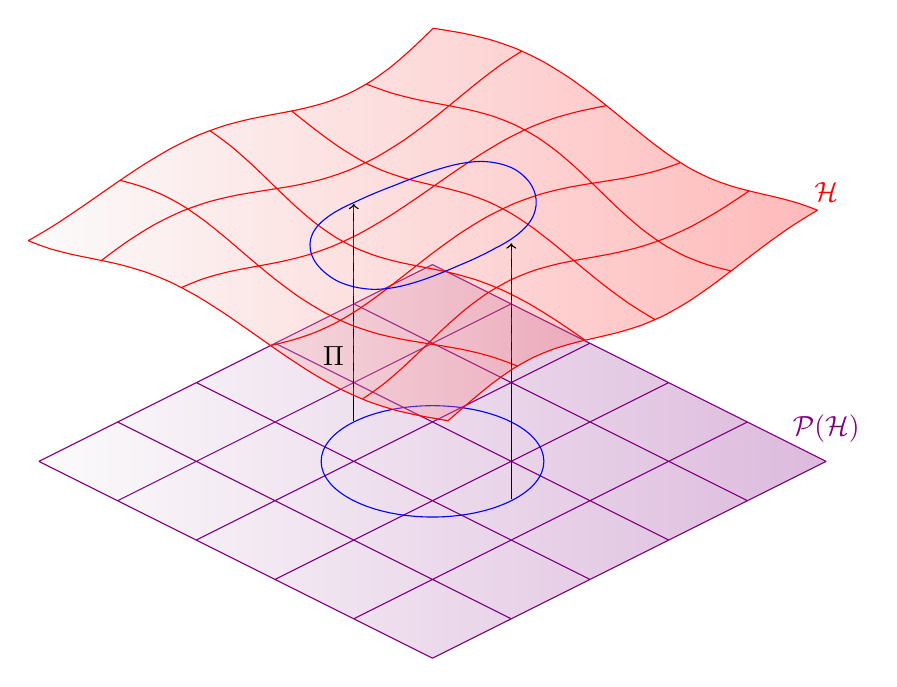
\begin{tikzpicture}[lattice/.cd,spacing/.initial=4,superlattice
  period/.initial=30,amplitude/.initial=3]  
  
     \begin{scope}[
            yshift=-83,every node/.append style={
            yslant=0.5,xslant=-1},yslant=0.5,xslant=-1
            ]
        % opaci
\begin{scope}[xshift=-3cm,yshift=-3cm]
	\shade[left color=gray!10,right color=violet!90,opacity=.30] (0,0) rectangle (5,5);
	\draw[violet] (0,0) grid (5,5);
    \draw[blue] (2.5,2.5) circle (1);
\end{scope} 
\end{scope} 


\draw[->] (-1,-2.9) -- (-1,-0.15) ;
\draw[->] (1,-3.9) -- (1,-0.65);
\begin{scope}[
            yshift=-83,every node/.append style={
            yslant=0.5,xslant=-1},yslant=0.5,xslant=-1
            ]
\begin{scope}
    \pgftransformnonlinear{\latticetilt}
\begin{scope}
    \pgftransformnonlinear{\latticetilt}
	%\fill[white] 
	\shade[left color=gray!10,right color=red!90,opacity=.30] (0,0) rectangle (5,5);
        
    \draw[red] (0,0) grid (5,5);
    \draw[blue] (2.5,2.5) circle (1);
\end{scope} 
\end{scope} 
\end{scope} 

\draw[->,dashed] (-1,-2.9) -- (-1,-0.15) node [pos=0.3,left] {$\Pi$};
\draw[->,dashed] (1,-3.9) -- (1,-0.65);


\node [red] at (5,0) {$\mathcal{H}$};
\node [violet] at (5,-3) {$\mathcal{P(H)}$};
\end{tikzpicture}
\end{document}



% Projection of circles onto a spherical surface
% Author: Mark Wibrow
\documentclass[border=10pt]{standalone}
\usepackage{tikz}
\usetikzlibrary{intersections}

\begin{document}

\begin{tikzpicture}[xscale=0.8,>=latex]


\begin{scope}[rotate = -80, shift={(2,-2)}]

% border of the surface2
\path[draw,name path=border3] (1,-4) to (3,5);
% border of the surface2
\path[draw,name path=border4] (6,-7) to (7,5);
% border of the surface2
\path[draw,name path=border5] (1,-4) to (6,-7);
% border of the surface2
\path[draw,name path=border6] (3,5) to (7,5);


% draw the surface2
\shade[top color=gray!10,bottom color=blue!90,opacity=.30] 
  (1,-4) to(3,5)  to (7,5)
 to (6,-7) to(1,-4);

\end{scope}



\begin{scope}[rotate = -80]
% border of the surface2
\path[draw,name path=border3] (1,-4) to[out=60,in=220] (3,5);
% border of the surface2
\path[draw,name path=border4] (6,-7) to[out=70,in=210] (7,5);
% border of the surface2
\path[draw,name path=border5] (1,-4) to[out=0,in=80] (6,-7);
% border of the surface2
\path[draw,name path=border6] (3,5) to[out=10,in=140] (7,5);


% draw the surface2
\shade[top color=gray!10,bottom color=red!90,opacity=.30] 
  (1,-4) to[out=60,in=220] (3,5)  to[out=10,in=140] (7,5)
 to[out=210,in=70] (6,-7) to[out=80,in=0] (1,-4);

\end{scope}

\end{tikzpicture}

\end{document}

% border of the surface1
\path[draw,name path=border1] (0,0) to[out=-10,in=150] (6,-2)--(12,1) --(5.5,3.2) -- cycle;
% border of the surface1
\path[draw,name path=border2] (12,1) to[out=150,in=-10] (5.5,3.2);
% border of the surface1
\path[draw,name path=line2] (5.5,3.7) -- (0,0);
% draw the surface1
\shade[left color=gray!10,right color=gray!70] 
  (0,0) to[out=-10,in=150] (6,-2) --  (12,1) to[out=150,in=-10] (5.5,3.7) -- cycle;
